% ============================================================
%  DISCOVERY CURRICULUM — Journey 1, Module 6
%  "Mathematical Modelling"
%  Compile with: pdflatex J1_M6.tex  (run twice for references)
% ============================================================

\documentclass[12pt, a4paper]{article}

\usepackage[a4paper, top=2.8cm, bottom=2.8cm, left=3.0cm, right=2.5cm, includeheadfoot, headheight=15pt]{geometry}
\usepackage{amsmath, amsthm}
\usepackage[charter, cal=cmcal]{mathdesign}
\usepackage[scaled=0.92]{helvet}
\usepackage{xcolor}
\usepackage{tcolorbox}
\tcbuselibrary{skins, breakable, theorems}
\usepackage{enumitem}
\usepackage{graphicx}
\usepackage{tikz}
\usetikzlibrary{arrows.meta, positioning, calc}
\usepackage{pgfplots}
\pgfplotsset{compat=1.18}
\usepackage{booktabs}
\usepackage{array}
\usepackage{fancyhdr}
\usepackage{titlesec}
\usepackage{parskip}
\usepackage{microtype}
\usepackage{hyperref}
\hypersetup{colorlinks=true, linkcolor=NavyBlue, urlcolor=NavyBlue}

% ── Colours ─────────────────────────────────────────────────
\definecolor{NavyBlue}{HTML}{1E3A8A}
\definecolor{MidBlue}{HTML}{2E6DA4}
\definecolor{Gold}{HTML}{D97706}
\definecolor{LightBlue}{HTML}{EFF6FF}
\definecolor{LightGold}{HTML}{FEF3C7}
\definecolor{DarkGrey}{HTML}{334155}
\definecolor{BoxGreen}{HTML}{F0FDF4}
\definecolor{SoftRed}{HTML}{FFF1F2}
\definecolor{SidebarGrey}{HTML}{F8FAFC}
\definecolor{WarnRed}{HTML}{FFF1F2}
\definecolor{EdgeRed}{HTML}{E11D48}

% ── Section formatting ───────────────────────────────────────
\titleformat{\section}{\Large\bfseries\color{NavyBlue}}{}{0em}{}[{\color{MidBlue}\vspace{2pt}\rule{\linewidth}{1.5pt}}]
\titleformat{\subsection}{\large\bfseries\color{MidBlue}}{}{0em}{}
\titleformat{\subsubsection}{\normalsize\bfseries\color{Gold}}{}{0em}{}

% ── Header / Footer ─────────────────────────────────────────
\pagestyle{fancy}
\fancyhf{}
\fancyhead[L]{\small\color{DarkGrey}\textit{Discovery Curriculum}}
\fancyhead[R]{\small\color{DarkGrey}\textit{Journey 1 $\cdot$ Module 6}}
\fancyfoot[C]{\small\color{MidBlue}\thepage}
\renewcommand{\headrulewidth}{0.4pt}

% ── Environments (tcolorbox Unification) ─────────────────────

% Puzzle box — opening problem
\newtcolorbox{puzzlebox}[1][]{
  enhanced, breakable,
  colback=NavyBlue!5, colframe=NavyBlue,
  boxrule=0pt, leftrule=2.5pt,
  sharp corners,
  left=12pt, right=10pt, top=10pt, bottom=10pt,
  before skip=14pt, after skip=10pt,
  #1
}

% Discovery box — moment of crystallisation
\newtcolorbox{discoverybox}[1][]{
  enhanced, breakable,
  colback=LightGold, colframe=Gold,
  boxrule=0pt, leftrule=2.5pt,
  sharp corners,
  left=12pt, right=10pt, top=10pt, bottom=10pt,
  before skip=14pt, after skip=10pt,
  #1
}

% Name box — formal definition reveal
\newtcolorbox{namebox}[1][]{
  enhanced, breakable,
  colback=LightBlue, colframe=MidBlue,
  boxrule=0.8pt,
  arc=4pt,
  left=12pt, right=10pt, top=10pt, bottom=10pt,
  before skip=14pt, after skip=10pt,
  #1
}

% Reflection box
\newtcolorbox{reflectionbox}[1][]{
  enhanced, breakable,
  colback=BoxGreen, colframe=DarkGrey!35,
  boxrule=0.8pt,
  arc=4pt,
  left=12pt, right=10pt, top=10pt, bottom=10pt,
  before skip=14pt, after skip=10pt,
  #1
}

% Thought provocation — inline philosophical aside
\newtcolorbox{thought}[1][]{
  enhanced, breakable,
  colback=SidebarGrey, colframe=Gold,
  boxrule=0pt, leftrule=1.5pt,
  sharp corners,
  left=10pt, right=10pt, top=7pt, bottom=7pt,
  before skip=10pt, after skip=10pt,
  #1
}

% Warning box
\newtcolorbox{warning}[1][]{
  enhanced, breakable,
  colback=WarnRed, colframe=EdgeRed!60,
  boxrule=0pt, leftrule=1.5pt,
  sharp corners,
  left=12pt, right=10pt, top=7pt, bottom=7pt,
  before skip=10pt, after skip=10pt,
  #1
}

% Problem counter
\newcounter{problem}
\newenvironment{problem}[1][]{%
  \refstepcounter{problem}%
  \par\vspace{6pt}%
  \noindent\textbf{\color{MidBlue}Problem \theproblem}%
  \ifx&#1&\else\ \textit{(#1)}\fi\textbf{.}\enskip
}{\par\vspace{4pt}}

% Deep problem counter
\newcounter{deepproblem}
\newenvironment{deepproblem}[1][]{%
  \refstepcounter{deepproblem}%
  \par\vspace{6pt}%
  \noindent\textbf{\color{NavyBlue}$\bigstar$\ Deep Problem \thedeepproblem}%
  \ifx&#1&\else\ \textit{(#1)}\fi\textbf{.}\enskip
}{\par\vspace{4pt}}

% Exercise counter
\newcounter{exercise}
\newenvironment{exercise}[1][]{%
  \refstepcounter{exercise}%
  \par\vspace{6pt}%
  \noindent\textbf{\color{Gold}Exercise \theexercise}%
  \ifx&#1&\else\ \textit{(#1)}\fi\textbf{.}\enskip
}{\par\vspace{4pt}}

\begin{document}
% ============================================================

% ── Cover ───────────────────────────────────────────────────
\thispagestyle{empty}
\begin{center}
{\small\color{MidBlue}\textbf{DISCOVERY CURRICULUM}\quad$\cdot$\quad\textbf{JOURNEY 1: REPRESENTATION}}

\vspace{0.6cm}
{\color{NavyBlue}\rule{\linewidth}{2pt}}
\vspace{0.5cm}

{\Huge\bfseries\color{NavyBlue}Module 6}\\[0.3cm]
{\LARGE\bfseries\color{MidBlue}Mathematical Modelling}\\[0.4cm]
{\color{Gold}\rule{0.4\linewidth}{1.2pt}}\\[0.4cm]
{\large\itshape\color{DarkGrey}
A model is a controlled lie.\\[0.15cm]
The art is knowing exactly what you are lying about.}

\vspace{1cm}
\begin{tabular}{rl}
\color{DarkGrey}\textbf{Journey}           & Journey 1 --- Representation \\[4pt]
\color{DarkGrey}\textbf{Module}            & 6 of 6 \textit{(final module of Journey 1)} \\[4pt]
\color{DarkGrey}\textbf{Prerequisites}     & Modules 1--5 (all of Journey 1) \\[4pt]
\color{DarkGrey}\textbf{You will discover} & The modelling cycle, dimensional analysis, model failure, fitting, validation \\[4pt]
\color{DarkGrey}\textbf{Format}            & 8 problems $+$ 3 deep problems $\approx$ 13--15 pages \\
\end{tabular}

\vspace{1cm}
{\color{NavyBlue}\rule{\linewidth}{2pt}}
\end{center}

\vspace{0.6cm}

\noindent\textbf{The closing module of Journey 1.}
You have spent five modules building languages: functions, graphs, sequences, recursion, exponential growth. Each language was developed in response to a specific problem. Now we step back and ask the foundational question that underlies all of them:

\medskip
\begin{center}
\itshape
When does a mathematical structure faithfully represent something in the world?\\
When does it mislead? And how do we tell the difference?
\end{center}

\medskip
This is not a philosophical indulgence. These questions determine whether bridges stand or collapse, whether drugs are approved or withdrawn, whether epidemics are contained or allowed to spread. Every person who applies mathematics to reality must answer them, continuously, with imperfect information.

\newpage

% ============================================================
\section{Part 1 \texorpdfstring{---}{--} The Puzzle}
% ============================================================

\begin{puzzlebox}
\textbf{The Opening Puzzle: Three Models of a Population.}

A wildlife ecologist is tracking the population of a species in a protected reserve. She has three candidate models, all consistent with the data from the first five years:

\medskip
\textbf{Model A:} $P(t) = 200 + 40t$ \hfill (linear growth)

\textbf{Model B:} $P(t) = 200 \cdot (1.15)^t$ \hfill (exponential growth)

\textbf{Model C:} $P(t) = \dfrac{2000}{1 + 9e^{-0.3t}}$ \hfill (logistic growth)

\medskip
The data so far:

\begin{center}
\begin{tabular}{ccccc}
\toprule
$t$ (years) & 0 & 1 & 2 & 3 & 4 \\
\midrule
$P$ (observed) & 200 & 232 & 270 & 315 & 363 \\
\bottomrule
\end{tabular}
\end{center}

\medskip
\textbf{Question 1.} Compute each model's prediction for $t = 0, 1, 2, 3, 4$. Which fits the data best?

\textbf{Question 2.} Project each model to $t = 10, 20, 50$. Do the predictions agree? Which is most realistic, and why?

\textbf{Question 3.} The reserve has a carrying capacity of 2000 animals due to limited food and territory. Which model encodes this constraint? What happens to the others at large $t$?
\end{puzzlebox}

\medskip
All three models are mathematically valid. All three are consistent with the same five data points. Yet they make wildly different predictions for the future. This is the central difficulty of modelling: the data you have never uniquely determines the model. Choosing between models requires assumptions, judgement, and knowledge of the underlying system that go beyond the numbers.

\begin{thought}
\textbf{All models are wrong.}
The statistician George Box wrote: \textit{``All models are wrong, but some are useful.''} This is not cynicism. It is clarity. A model is a deliberate simplification. It omits friction, noise, individual variation, external shocks, and a thousand other factors. The question is never whether a model is true --- it is not. The question is whether it is useful for the purpose at hand, over the domain of interest, with an understood margin of error. A map of Nairobi that shows only major roads is wrong in the sense that it omits thousands of streets. It is useful if you are driving between districts. It is useless if you are looking for a specific house. The model's fitness depends entirely on the question you are asking.
\end{thought}

% ============================================================
\section{Part 2 \texorpdfstring{---}{--} Exploration}
% ============================================================

\subsection{Step 1: The modelling cycle}

Mathematical modelling is not a single act. It is a cycle, repeated until the model is good enough for its purpose.

\begin{center}
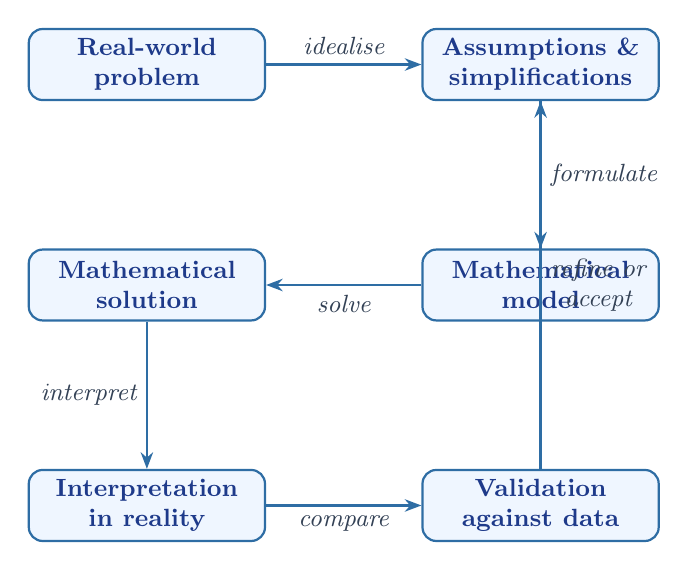
\begin{tikzpicture}[
  box/.style={rectangle, rounded corners=5pt, draw=MidBlue, thick,
              fill=LightBlue, minimum width=3cm, minimum height=0.9cm,
              align=center, font=\small\bfseries\color{NavyBlue}},
  arr/.style={-{Stealth[length=6pt]}, MidBlue, thick},
  lbl/.style={font=\small\itshape, color=DarkGrey}
]
\node[box] (real)   at (0, 0)    {Real-world\\problem};
\node[box] (assume) at (5, 0)    {Assumptions \&\\simplifications};
\node[box] (math)   at (5, -2.8) {Mathematical\\model};
\node[box] (solve)  at (0, -2.8) {Mathematical\\solution};
\node[box] (interp) at (0, -5.6) {Interpretation\\in reality};
\node[box] (valid)  at (5, -5.6) {Validation\\against data};

\draw[arr] (real)   -- node[above, lbl] {idealise} (assume);
\draw[arr] (assume) -- node[right, lbl] {formulate} (math);
\draw[arr] (math)   -- node[below, lbl] {solve} (solve);
\draw[arr] (solve)  -- node[left,  lbl] {interpret} (interp);
\draw[arr] (interp) -- node[below, lbl] {compare} (valid);
\draw[arr] (valid)  -- node[right, lbl, align=center] {refine or\\accept} (assume);
\end{tikzpicture}
\end{center}

\begin{problem}
\label{prob:modelling_cycle}
Apply the modelling cycle to each of the following situations. For each: identify the real-world system, state the simplifying assumptions explicitly, write a mathematical model, solve or analyse it, and describe at least two ways the model might fail.

\begin{enumerate}[label=(\alph*), topsep=2pt]
  \item A stone is dropped from a 100-metre building. Model the time it takes to hit the ground.
  \item A disease spreads in a school of 800 students. Initially 5 are infected. Model the spread over 10 days.
  \item A rumour spreads through a social network. The network has the structure of the seven-town graph from Module~3. Model how long it takes for the rumour to reach every node.
  \item A country's GDP grows by 3\% per year. Model GDP over 30 years. Identify the most dangerous assumption.
\end{enumerate}
\end{problem}

\subsection{Step 2: Dimensional analysis --- the hidden constraint}

Before writing any equation, there is a powerful check you should always apply: \emph{are the units consistent?}

\begin{problem}
\label{prob:dimensions}
Every physical quantity has dimensions. For example: speed has dimensions of $[\text{length}]/[\text{time}]$, written $[L/T]$. Force has dimensions $[M L / T^2]$ (mass times acceleration).
\begin{enumerate}[label=(\alph*), topsep=2pt]
  \item Determine the dimensions of: energy, pressure, density, frequency, electrical charge.
  \item The period $\tau$ of a simple pendulum depends on its length $\ell$ and the gravitational acceleration $g$. Assume $\tau = C \cdot \ell^a \cdot g^b$ for some constants $C, a, b$. Use dimensional analysis to find $a$ and $b$. (You cannot determine $C$ this way --- why not?)
  \item A physicist writes the equation $v = at + \frac{1}{2}at^2$ for the velocity of an accelerating object. Is this equation dimensionally consistent? If not, correct it.
  \item The formula for the energy of a photon is $E = hf$ where $f$ is frequency. What are the dimensions of Planck's constant $h$?
  \item Why is it impossible for a valid physical equation to state that a length equals a time? What does this tell you about the structure of physical law?
\end{enumerate}
\end{problem}

\begin{thought}
\textbf{Dimensional analysis as a superpower.}
In 1999, the Mars Climate Orbiter was lost because one engineering team used metric units (newton-seconds) and another used imperial units (pound-force seconds) for the same thruster data. The spacecraft entered the Martian atmosphere at the wrong angle and burned up. Total cost: \$327 million. The error would have been caught by a routine dimensional check of the telemetry data. Dimensional analysis is not a formality. It is a constraint imposed by the structure of physical reality. Any equation whose dimensions do not balance is guaranteed to be wrong. This sounds obvious. It is violated constantly.
\end{thought}

\subsection{Step 3: Fitting models to data}

\begin{problem}
\label{prob:fitting}
You have collected the following data on the spread of a disease. $I(t)$ is the number of infected individuals on day $t$:

\begin{center}
\begin{tabular}{ccccccc}
\toprule
$t$ & 0 & 2 & 4 & 6 & 8 & 10 \\
\midrule
$I(t)$ & 5 & 13 & 34 & 88 & 226 & 580 \\
\bottomrule
\end{tabular}
\end{center}

\begin{enumerate}[label=(\alph*), topsep=2pt]
  \item Plot the data. Does it look linear, exponential, or logistic?
  \item To test for exponential growth, compute $\ln I(t)$ for each data point. Plot $\ln I$ against $t$. What shape do you see?
  \item If $I(t) = I_0 e^{kt}$, then $\ln I(t) = \ln I_0 + kt$ --- a linear relationship. Use two data points to estimate $k$ and $I_0$.
  \item A school has 1200 students. Does the exponential model make sense for all time? When must it break down?
  \item The \textbf{SIR model} divides the population into Susceptible ($S$), Infected ($I$), and Recovered ($R$). Infections happen when $S$ and $I$ meet; recoveries happen at a fixed rate. Write down (informally) the rules governing how $S$, $I$, $R$ change over time. What does the system look like when almost everyone is recovered?
\end{enumerate}
\end{problem}

\begin{problem}
\label{prob:least_squares}
You have five data points $(x_i, y_i)$ and you want to fit a line $y = mx + c$.

\begin{center}
\begin{tabular}{cccccc}
\toprule
$x$ & 1 & 2 & 3 & 4 & 5 \\
\midrule
$y$ & 2.1 & 3.9 & 6.2 & 7.8 & 10.1 \\
\bottomrule
\end{tabular}
\end{center}

\begin{enumerate}[label=(\alph*), topsep=2pt]
  \item Plot the data. Does a linear model look reasonable?
  \item For a given line $y = mx + c$, the \textbf{residual} at point $i$ is $r_i = y_i - (mx_i + c)$. Compute residuals for $m = 2, c = 0$.
  \item The \textbf{least squares} criterion chooses $m$ and $c$ to minimise $\sum_{i=1}^5 r_i^2$. Explain geometrically why we minimise the sum of \emph{squared} residuals rather than the sum of residuals.
  \item The least squares solution satisfies:
  \[
    m = \frac{n\sum x_i y_i - \sum x_i \sum y_i}{n\sum x_i^2 - \left(\sum x_i\right)^2}, \qquad
    c = \frac{\sum y_i - m\sum x_i}{n}.
  \]
  Apply this to the data above to find the best-fit line.
  \item The formula in (d) is a formula for a function: it takes data as input and returns parameters as output. In Journey~3 you will see that least squares is fundamentally a projection in a vector space. For now: does the formula look like it could be written as a matrix equation?
\end{enumerate}
\end{problem}

\begin{thought}
\textbf{What does ``best fit'' mean?}
The least squares criterion --- minimise the sum of squared errors --- is not the only possible criterion. You could minimise the sum of absolute errors, or the maximum error, or some weighted combination. The choice of criterion encodes assumptions about what kind of errors matter. Least squares has a beautiful theoretical justification: if the errors are normally distributed (the bell curve from Module~5), then least squares gives the most probable parameter values. This connection between optimisation and probability --- between fitting and believing --- is one of the deepest threads in statistics, and it leads directly to Bayesian inference in Journey~5.
\end{thought}

\subsection{Step 4: When models break --- and what that means}

\begin{problem}
\label{prob:model_failure}
Each of the following is a famous case where a mathematical model gave dangerously wrong predictions. For each: identify the model used, explain what it got wrong, and describe the real-world consequences.

\begin{enumerate}[label=(\alph*), topsep=2pt]
  \item \textbf{The 2008 financial crisis.} Banks used models based on the assumption that mortgage defaults across the US were largely independent events. What is the independence assumption? What happens when it fails? (Hint: think about correlation during a nationwide recession.)

  \item \textbf{Chernobyl.} The reactor safety model assumed that a certain type of test could be run safely because the reactor had always behaved stably at high power. What kind of reasoning is this? What did it fail to account for?

  \item \textbf{Phlogiston theory.} For a century, chemists modelled combustion as the release of a substance called phlogiston. The model made correct predictions within its domain. Then it was replaced entirely. What does this tell us about the relationship between predictive success and truth?

  \item \textbf{Newtonian gravity.} Newton's model of gravity was extraordinarily accurate for two centuries. Then it was found to be wrong in certain regimes (near very massive objects, at very high speeds). Was Newton's model false? Was it useful? How should we think about a model that works perfectly in one regime and fails in another?
\end{enumerate}
\end{problem}

\begin{warning}
\textbf{The most dangerous kind of model failure.}
A model that is always wrong is quickly discarded. A model that is usually right and occasionally catastrophically wrong is far more dangerous, because it earns trust before it destroys it. This is the pattern in financial models (correct 999 days out of 1000, catastrophic on day 1000), in structural engineering models (correct for every load until the one that causes collapse), and in epidemiological models (correct for endemic disease, wrong for a novel pandemic). The lesson is not to distrust models --- it is to understand their domain of validity with precision, and to remain genuinely uncertain at the boundaries.
\end{warning}

\begin{problem}
\label{prob:logistic}
Return to the logistic model from the opening puzzle: $P(t) = \dfrac{K}{1 + Ae^{-rt}}$, where $K$ is the carrying capacity, $r$ is the growth rate, and $A$ is determined by the initial condition.
\begin{enumerate}[label=(\alph*), topsep=2pt]
  \item Show that $P(0) = K/(1+A)$. Use this to express $A$ in terms of $P(0)$ and $K$.
  \item Show that as $t \to \infty$, $P(t) \to K$. Show that as $t \to -\infty$, $P(t) \to 0$.
  \item Find the value of $t$ at which $P(t) = K/2$ (the inflection point). What is the growth rate $P'(t)$ at this point?
  \item The logistic model assumes $K$ is fixed. List three biological mechanisms that could change $K$ over time. What would the model look like if $K = K(t)$?
  \item In Module~4, you encountered the logistic \emph{map} $x_{n+1} = rx_n(1-x_n)$. This is the discrete-time version of the logistic model. When $r$ is large, it produces chaos. Does the continuous logistic model also produce chaos? What is different about the continuous case?
\end{enumerate}
\end{problem}

\begin{problem}
\label{prob:modelling_design}
Design your own model for one of the following situations. Explicitly state your assumptions, write the mathematical structure, identify the variables and parameters, and describe how you would validate the model.

\begin{enumerate}[label=(\alph*), topsep=2pt]
  \item The spread of a new idea through a population (not a disease --- people can forget ideas, and can be exposed multiple times).
  \item The traffic flow on a single-lane road between two cities.
  \item The time it takes for a new technology to be adopted by a population (think about how smartphones spread from 2007 onwards).
  \item The number of species on an island as a function of the island's size and distance from the mainland.
\end{enumerate}

There is no single correct answer. You will be assessed on whether your model: (1) is internally consistent, (2) encodes the key mechanisms, (3) makes testable predictions, (4) has clearly identified limitations.
\end{problem}

\begin{thought}
\textbf{The unreasonable effectiveness of mathematics.}
In 1960, the physicist Eugene Wigner wrote an essay titled ``The Unreasonable Effectiveness of Mathematics in the Natural Sciences.'' His central puzzle: why do abstract mathematical structures --- developed with no thought of physical application --- turn out to describe the physical world with extraordinary precision? The complex numbers were invented as an algebraic convenience. They turn out to govern quantum mechanics. Non-Euclidean geometry was developed as a logical exercise. It turns out to describe the geometry of spacetime. The Fourier transform was invented to solve a heat equation. It turns out to govern signal processing, quantum mechanics, and the structure of the universe at every scale.

Wigner had no explanation. Neither does anyone else. Some say mathematics is so flexible that any physical theory can be expressed in it. Some say the universe is fundamentally mathematical. Some say we are so good at finding mathematical patterns that we see them even where they are approximate. This is one of the deepest open questions in the philosophy of science, and it is not going away.
\end{thought}

% ============================================================
\section{Part 3 \texorpdfstring{---}{--} Discovery}
% ============================================================

\begin{discoverybox}
\textbf{What have we built?}

This module has made explicit what every previous module in Journey~1 was implicitly practising.

\medskip
\textbf{Modelling is a cycle, not a formula.} You go from reality to assumptions to mathematics to solution to interpretation to validation --- and then back to assumptions, refined by what you found. The cycle terminates when the model is good enough, not when it is perfect.

\medskip
\textbf{Assumptions are the hidden architecture.} Every model encodes assumptions about what matters and what doesn't. A linear model assumes constant rate of change. An exponential model assumes proportional growth. A logistic model assumes a carrying capacity. None of these is true in the strict sense --- they are choices, and they must be owned explicitly.

\medskip
\textbf{Model failure is informative.} When a model breaks down, it is telling you something about the world that your assumptions missed. Newton's gravity was not merely wrong --- its failure in extreme regimes pointed directly at the missing structure that Einstein supplied.

\medskip
\textbf{Before closing Journey~1:} Look back at Modules 1--5. In each module, a mathematical structure was introduced as a solution to a problem. Now identify, for each structure, what it is a \emph{model} of. What are its assumptions? Where does it break down?
\end{discoverybox}

% ============================================================
\section{Part 4 \texorpdfstring{---}{--} Naming the Ideas}
% ============================================================

\begin{namebox}
\textbf{The modelling vocabulary.}

A \textbf{mathematical model} is a set of mathematical structures (functions, equations, graphs, sequences) together with an interpretation that assigns real-world meaning to the variables and parameters.

\medskip
A model has:
\begin{itemize}[topsep=4pt, noitemsep]
  \item \textbf{Variables}: quantities that change (population, time, temperature).
  \item \textbf{Parameters}: quantities treated as fixed within the model but that can be adjusted (growth rate $k$, carrying capacity $K$).
  \item \textbf{Assumptions}: simplifications that make the model tractable (no immigration, no predators, constant environment).
  \item \textbf{Domain of validity}: the range of conditions under which the model makes reliable predictions.
\end{itemize}
\end{namebox}

\begin{namebox}
\textbf{Key models encountered in Journey 1.}

\begin{center}
\renewcommand{\arraystretch}{1.4}
\begin{tabular}{l l l}
\toprule
\textbf{Model} & \textbf{Mathematical form} & \textbf{Key assumption} \\
\midrule
Linear & $y = mx + c$ & Constant rate of change \\
Exponential & $P(t) = P_0 e^{kt}$ & Growth proportional to size \\
Logistic & $P(t) = K/(1+Ae^{-rt})$ & Growth limited by carrying capacity \\
Power law & $y = ax^b$ & Scale-free relationship \\
Recursive & $a_n = f(a_{n-1})$ & Next state depends only on current \\
Graph model & $G = (V, E)$ & Relationships encoded as connections \\
\bottomrule
\end{tabular}
\end{center}
\end{namebox}

\begin{namebox}
\textbf{Dimensional analysis.}

Every term in a valid physical equation must have the same dimensions. The \textbf{Buckingham $\pi$ theorem} states that any physically meaningful equation relating $n$ quantities with $k$ independent dimensions can be written as a relationship between $n - k$ dimensionless groups. Dimensional analysis can often determine the form of a physical law up to a dimensionless constant.
\end{namebox}

% ============================================================
\section{Part 5 \texorpdfstring{---}{--} Deep Problems}
% ============================================================

\begin{deepproblem}[The SIR model]
The \textbf{SIR model} for epidemic spread divides a population of size $N$ into three compartments: Susceptible $S$, Infected $I$, Recovered $R$, with $S + I + R = N$. The dynamics are governed by:
\[
  \frac{dS}{dt} = -\beta S I, \qquad
  \frac{dI}{dt} = \beta S I - \gamma I, \qquad
  \frac{dR}{dt} = \gamma I,
\]
where $\beta$ is the transmission rate and $\gamma$ is the recovery rate.
\begin{enumerate}[label=(\alph*)]
  \item Verify that $\frac{d}{dt}(S + I + R) = 0$, confirming the total population is conserved.
  \item The \textbf{basic reproduction number} is $R_0 = \beta N / \gamma$. Show that the epidemic grows (i.e.\ $dI/dt > 0$) when $S > \gamma/\beta$, and relate this to $R_0$.
  \item Explain in plain language what $R_0 > 1$ means biologically. Why is reducing $\beta$ (through social distancing) or increasing $\gamma$ (through treatment) equivalent strategies for controlling the epidemic?
  \item The model assumes homogeneous mixing: every pair of individuals is equally likely to interact. This is wrong in every real population. What graph-theoretic structure would replace this assumption? How would the epidemic dynamics change if the contact network were a star graph versus a complete graph?
  \item \textit{(Research question.)} The SIR model predicts that the epidemic ends not because everyone is infected, but because $S$ falls below the threshold $\gamma/\beta$. The fraction of the population that escapes infection is called the \emph{herd immunity threshold}. Derive an equation for this fraction in terms of $R_0$.
\end{enumerate}
\end{deepproblem}

\begin{deepproblem}[Least squares as projection]
This problem previews a result that will be proved fully in Journey~3.

Let $\mathbf{y} = (y_1, \ldots, y_n)^T$ be a vector of observations and let $X$ be the $n \times 2$ matrix whose rows are $(1, x_i)$.
\begin{enumerate}[label=(\alph*)]
  \item The linear model predicts $\hat{\mathbf{y}} = X\boldsymbol{\beta}$ where $\boldsymbol{\beta} = (c, m)^T$. Write out $X\boldsymbol{\beta}$ explicitly.
  \item The least squares criterion is $\min_{\boldsymbol{\beta}} \|\mathbf{y} - X\boldsymbol{\beta}\|^2$. What geometric object is $\{X\boldsymbol{\beta} : \boldsymbol{\beta} \in \mathbb{R}^2\}$?
  \item The minimum is achieved when $\mathbf{y} - \hat{\mathbf{y}}$ is perpendicular to every column of $X$. Write this condition as $X^T(\mathbf{y} - X\boldsymbol{\beta}) = 0$ and solve for $\boldsymbol{\beta}$.
  \item The solution $\boldsymbol{\hat\beta} = (X^TX)^{-1}X^T\mathbf{y}$ is the \textbf{normal equation}. Verify that it reproduces the formulas in Problem~\ref{prob:least_squares}(d).
  \item Geometrically: the best-fit line is found by \emph{projecting} the observation vector $\mathbf{y}$ onto the column space of $X$. What does this say about the nature of fitting --- is it fundamentally an algebraic or a geometric operation?
\end{enumerate}
\end{deepproblem}

\begin{deepproblem}[Scaling laws in nature]
Many quantities in biology and physics follow \textbf{power laws}: $y \propto x^b$ for some exponent $b$.
\begin{enumerate}[label=(\alph*)]
  \item The metabolic rate $M$ (energy used per unit time) of mammals scales with body mass $m$ as $M \propto m^{3/4}$. This is called \textbf{Kleiber's law}. Verify: a mouse weighs 20 g and has metabolic rate 0.28 W; an elephant weighs 4000 kg and has metabolic rate 2890 W. Does the $3/4$ power law hold approximately?
  \item If $y = ax^b$, then $\log y = \log a + b \log x$ is linear in $\log x$. Use this to explain how you would detect a power law from data.
  \item The exponent $b = 3/4$ in Kleiber's law has been derived from a fractal model of the circulatory system. The argument is: the circulatory network fills 3-dimensional space but is constrained by 2-dimensional surfaces (vessel walls). The exponent $3/4$ is a dimensionless combination of 2 and 3. Does this derivation feel convincing? What assumptions does it make?
  \item Zipf's law states that the frequency of the $r$-th most common word in a language is proportional to $1/r$. The same law appears in city population rankings, earthquake magnitudes, and income distributions. Verify Zipf's law approximately for English using the approximate frequencies: ``the'' appears $\sim 7\%$ of the time, ``of'' $\sim 3.5\%$, ``and'' $\sim 2.3\%$. Does this make you more or less confident that the law reflects a deep truth?
  \item \textit{(Open question.)} Why do power laws appear in so many unrelated systems? Two competing explanations are: (1) there is a deep mathematical reason (perhaps related to self-similarity or scale-invariance), or (2) power laws are so flexible that almost any fat-tailed distribution looks like a power law on a log-log plot. Argue for each position.
\end{enumerate}
\end{deepproblem}

% ============================================================
\section{Part 6 \texorpdfstring{---}{--} Reflection}
% ============================================================

\begin{reflectionbox}
\textbf{Final reflection for Journey 1.}

This is the end of Journey~1. Before you begin Journey~2, spend time with the following questions. They are designed to consolidate not just what you have learned but how you have learned to think.

\begin{enumerate}
  \item \textbf{On the modelling cycle.} Choose one model from any of Modules 1--5 --- the exponential population model, the function $d = 15t$, the Fibonacci recursion, the logistic map, anything. Write out the full modelling cycle for it: what real-world problem motivated it, what assumptions it encodes, what predictions it makes, and at least two ways it fails.

  \item \textbf{On assumptions.} Every mathematical structure you have met in Journey~1 is built on assumptions that are false in the strict sense. The function $d=15t$ assumes constant speed. The graph model assumes connections are binary (you are either connected or not). The logistic model assumes a fixed carrying capacity. Write a short paragraph: is it a problem that mathematical models are built on false assumptions? Can something be built on a false foundation and still be useful, or even true?

  \item \textbf{On Wigner's puzzle.} Wigner asked why abstract mathematics describes physical reality so well. After completing Journey~1, what is your best answer? Is it that we design mathematics to fit the world? Or that we notice only the cases where it fits? Or something else?

  \item \textbf{On what you have discovered.} Look back at the five modules before this one. In each module, you encountered an idea before it was named. Write down the five ideas, the problems that forced them into existence, and the names they were eventually given. This is your record of five genuine discoveries.

  \item \textbf{Looking ahead.} Journey~2 studies the mathematics of continuous change: derivatives, integrals, and differential equations. You have already met the key idea in Module~5: $e^x$ is its own rate of change. What do you think the derivative of a function means, before you are taught the definition? Write it down now. At the end of Journey~2, come back and compare.
\end{enumerate}
\end{reflectionbox}

% ============================================================
\section{Journey 1 \texorpdfstring{---}{--} Closing Summary}
% ============================================================

\begin{namebox}
\textbf{What Journey 1 built.}

\medskip
\begin{center}
\renewcommand{\arraystretch}{1.5}
\begin{tabular}{l l l}
\toprule
\textbf{Module} & \textbf{Core discovery} & \textbf{What it enabled} \\
\midrule
1 & Functions & A reliable language for rules between sets \\
2 & Inverse functions, function spaces & Reversibility; functions as objects \\
3 & Graphs and adjacency matrices & Structure without geometry \\
4 & Sequences, limits, recursion & The meaning of ``approaching a value'' \\
5 & $e^x$, logarithms, Euler's identity & Continuous growth; complex exponentials \\
6 & The modelling cycle & When and how mathematics touches reality \\
\bottomrule
\end{tabular}
\end{center}

\medskip
Every idea in this table will reappear in Journeys 2--7, usually in a deeper form. Functions reappear as differentiable maps, as operators on Hilbert spaces, as morphisms in categories. Sequences reappear as solutions to differential equations. The exponential function reappears in the solution to every linear ODE, in the Fourier and Laplace transforms, and in quantum mechanics. Graphs reappear as the structure underlying Markov chains, neural networks, and algebraic topology.

You have not finished these ideas. You have begun them.
\end{namebox}

\vspace{1.4cm}
\begin{center}
{\color{Gold}\rule{0.6\linewidth}{1.2pt}}\\[8pt]
{\large\bfseries\color{NavyBlue} End of Journey 1: Representation}\\[6pt]
{\normalsize\color{DarkGrey}\itshape
Six modules. Six discoveries. One language for describing structure.}\\[10pt]
{\color{Gold}\rule{0.6\linewidth}{1.2pt}}\\[10pt]
{\small\color{DarkGrey}Continue to: \textbf{Journey 2 --- Change: Inventing Calculus}}\\[4pt]
{\small\color{DarkGrey}\itshape
``The calculus is the greatest aid we have to the application of physical truth.''\\
\upshape --- William Fogg Osgood}
\end{center}

\end{document}